
\chapter{Funkcionální analýza a numerické metody}
\section{Míra a integrál}
\textit{objem a míra množiny, měřitelné množiny a funkce, Lebesgueúv integrál, záměna limitného přechodu a integrace}
\subsection{Míra na $\mathbb{R}$ a $\mathbb{R}^n$}
Míra je zobecněný pojem pro velikost množiny. Míra množiny $M$ v $\mathbb{R}^n$ je zobrazení, které každé množině $M$ ze systému měřitelných množin reálných čísel přiřadí číslo $m(M)\in \langle0,\infty\rangle$ udávající její velikost. Pro n=1 je míra zobecněním délky, pro n=2 plošného obsahu, pro n=3 objemu.  

Každou neprázdnou otevřenou podmnožinu $\mathbb{R}$ lze napsat jako sjednocení
konečně nebo spočetně mnoha disjunktních otevřených intervalů, tj. je-li $G\subset \mathbb{R}$ otevřená, potom existuje konečně nebo spočetně mnoho navzájem disjunktních otevřených intervalů $I_k =(a_k, b_k)$, přičemž $-\infty\leq a_k<b_k\leq \infty$, takových, že $G = \cup_kI_k$.
\begin{definition}
Míra otevřené množiny $G=\cup_k I_k$ je součet $m(G)=\sum_k(b_k-a_k)$ délek disjunktních intervalů $I_K=(a_k,b_k)$, které ji vytvářejí. Míra prázdné množiny je $m(\emptyset)=0$.
\end{definition}
\begin{definition}
Buď $F$ uzavřená omezená množina ležící v intervalu $I_K=(-K,K)$. Potom její míra je doplněk míry otevřené množiny $I_K \setminus F$ v $I_K$, tj. položíme
\begin{align*}
m(F) = m(I_K) - m(I_K \setminus F) = 2K - m(I_K\setminus F).
\end{align*}
\end{definition}
\begin{definition}
Buď $A$ podmnožinou intervalu $I_K=(-K,K)$. Potom\\
a) \textit{vnější míra} množiny $A$ je infimum měr otevřených množin obsahujících $A$, tj. 
\begin{align*}
m^*(A) = inf\{ m(G)|\,G \supset A,\,G-\text{otevřená}\}.
\end{align*}
Tímto vztahem definujeme i vnější míru neomezené množiny $A$.\\
b) \textit{vnitřní míra} omezené množiny $A$ je supremum měr uzavřených podmnožin $A$, tj. 
\begin{align*}
m_*(A)=sup\{m(F)|\,F\subset A,\,F-\text{uzavřená} \}.
\end{align*}
\end{definition}
\begin{definition}[Míra omezené množiny]
Buď $A\subset I_K=(-K,K).$\\
a)Množinu $A$ nazveme měřitelnou, jestliže vnitřní a vnější míra dávají stejnou hodnotu, kterou prohlásíme za \textit{míru} množiny $A$ a označíme symbolem $m(A)$:
\begin{align*}
m(A)=m^*(A)=m_*(A)
\end{align*}
b) Množina jejíž míra je nula se nazývá \textit{nulová množina}.
\end{definition}
\begin{definition}[Míra neomezené množiny]
Množina $A\subset\mathbb{R}$ je \textit{měřitelná}, pokud je měřitelný její průnik s každým intervalem $I_k(-k,k)$, tj. $A$ je měřitelná pokud pro každé $k\in\mathbb{N}$ množina $A_k=A\cap I_k$ je měřitelná.
\\Míra množiny $A$ je limita měr $A_k$, tj. 
\begin{align*}
m(A)=\lim_{k\rightarrow\infty}m(A\cap I_k).
\end{align*}
\end{definition}
Symbolem $\mathscr{M}$ označujeme systém měřitelných množin na $\mathbb{R}$.
Pozn. Každá spočetná množina je měřitelná a má míru nula. Příklad nespočetné množiny s mírou nula je například Cantorovo diskontinuum.
\subsection{Prostor s mírou} 
\begin{definition}
Nechť $X$ je základní prostor, tj. libovolná neprázdná množina. $\mathscr{S}$ je $\sigma$-algebra podmnožin $X$, tj. systém podmnožin základního prostoru $X$
splňující následující tři axiomy:
\begin{itemize}
\item systém obsahuje prázdnou množinu, tj. $\emptyset\in\mathscr{S}$,
\item systém je uzavřen na doplňky, tj. $A \in\mathscr{S}\Rightarrow X\setminus A\in\mathscr{S}$,
\item systém je uzavřen na spočetná sjednocení, tj. $A_i\in \mathscr{S}\,,i\in I\subset\mathbb{N}\Rightarrow \cup_{i\in I} A_i \in \mathscr{S}$.
\end{itemize}
Množiny ze systému $\mathscr{S}$ se nazývají měřitelné množiny. Dále nechť množinová funkce $\mu:\mathscr{S}\rightarrow \langle 0,\infty\rangle$ zvaná míra na $X$ je $\sigma$-aditivní, tj. pro spočetný
systém navzájem disjunktních množin $A_i \in \mathscr{S}\,,i\in I$, platí rovnost 
\begin{align*}
\mu(\cup_{i\in I} A_i)=\sum_{i\in I} \mu(A_i).
\end{align*}
Pak trojici $(X, \mathscr{S}, \mu)$ nazýváme prostor s mírou $\mu$.
\end{definition}

\begin{definition}
Buď $(X, \mathscr{S}, \mu)$ prostor s mírou. Potom míru $\mu$ nazveme
\begin{itemize}
\item \textit{konečnou}, jestliže míra celého prostoru je  konečná, tj. $\mu(X)<\infty$.
\item $\sigma$\textit{-konečnou}, pokud celý prostor lze napsat jako sjednocení spočetně mnoha množin s konečnou mírou, tj. existují $M_i\in \mathscr{S}\,,\mu(M_i)<\infty$, a $X=\cup_i M_i.$
\item \textit{úplnou}, jestliže každá podmnožina nulové množiny je měřitelná a nulová, tj. jestliže $B\in\mathscr{S}, \mu(B)=0$, potom $\forall A\subset B$ platí $A\in \mathscr{S}$ a $\mu(A)=0.$
\end{itemize}
\end{definition}
\begin{theorem}
Systém množin $\mathscr{M}$, tj. systém měřitelných množin na $\mathbb{R}$, s mírou $m$ splňují: 
\begin{itemize}
\item $\mathscr{M}$  je $\sigma$-algebra na $\mathbb{R}$.
\item $m$ je míra na $\mathscr{M}$. Navíc $m$ je $\sigma$-aditivní, $\sigma$-konečná, úplná a nezávislá na posunutí. 
\item Míra intervalu se shoduje s jeho délkou, tj. $m((a,b))=b-a$.
\item Aby $m$ zůstala nezávislá na posunutí, nelze ji rozšířit na větší $\sigma$-algebru než $\mathscr{M}$.
\end{itemize} 
\end{theorem}
\subsection{Měřitelné a integrovatelné funkce na $\mathbb{R}$}
\begin{definition}
Buď $\mathscr{M}$systém měřitelných podmnožin $\mathbb{R}$ a $f:\mathbb{R}\rightarrow \mathbb{R}^*$, kde $\mathbb{R}^*=\mathbb{R}\cup\{-\infty,\infty\}$.\\
a) \textit{Hladinová množina} funkce $f$ pro $\alpha\in \mathbb{R}$ je množina všech $x$, ve kterých hodnoty $f(x)$ přesáhnou $\alpha$. Tuto množinu označíme $E(f>\alpha)$, tj.
\begin{align*}
E(f>\alpha)=\{x\in \mathbb{R}|\,f(x)>\alpha\}.
\end{align*} 
Obecně pro interval nebo množinu $I\subset\mathbb{R}$ definujeme \textit{zobecněnou hladinovou množinu}
\begin{align*}
E(f\in I)=\{x\in \mathbb{R}|\,f(x)\in I\}=f^{-1}(I).
\end{align*}
b) Funkci $f$ nazveme \textit{měřitelnou}, jestliže její hladinové množiny jsou měřitelné, tj. $E(f>\alpha)\in \mathscr{M}$ pro všechna $\alpha\in \mathbb{R}$.
\end{definition}
Množinu všech měřitelných funkcí $f:\mathbb{R}\rightarrow\mathbb{R}^*$ značíme $\Lambda(\mathbb{R}).$
\begin{definition}
Řekneme, že nezáporná funkce $f$ na $\mathbb{R}$ je \textit{jednoduchá}, právě když je měřitelná a nabývá konečně mnoha hodnot. 
\end{definition}
Funkce $f$ je jednoduchá, právě když existuje konečně mnoho kladných konstant $c_1,\ldots c_k$ a disjunktních měřitelných množin $A_1,\ldots,A_k$ takových, že 
\begin{align*}
f(x)=\sum_{i=1}^k c_i\cdot \chi_{A_i}(x),
\end{align*}
kde $\chi_{A}(x)$ je charakteristická funkce množiny $A$, tj. $\chi_{A}(x)=1$ pro $x\in A$ a $\chi_{A}(x)=0$ pro $x\notin A$.
\begin{theorem}
Každou nezápornou měřitelnou funkci lze napsat jako bodovou limitu neklesající posloupnosti jednoduchých funkcí, tj. existuje neklesající posloupnost jednoduchých funkcí $\varphi_n(x)$ takových, že po každé $x$ platí:
\begin{align*}
\varphi_n(x)\rightarrow f(x) \text{ pro } n\rightarrow\infty.
\end{align*}
\end{theorem}
\subsection{Lebesgueův integrál}
\begin{definition}[Lebesgueův integrál]Zavedení\\
a) Integrál z jednoduché funkce $\varphi(x)=\sum_{i=1}^k c_i\cdot  \chi_{A_i}$, kde $c_i>0$ a $A_i$ jsou měřitelné disjunktní množiny, je součet (může být i nekonečno)
\begin{align*}
\int_\mathbb{R}\varphi(x)dx=\sum_{i=1}^k c_i \cdot m(A_i).
\end{align*}
b) Integrál z nezáporné měřitelné funkce $f(x)$ je limita
\begin{align*}
\int_\mathbb{R}f(x)dx=\lim_{k\rightarrow\infty}\int_\mathbb{R}\varphi_k(x)dx,
\end{align*}
kde $\{\varphi_k\}$ je neklesající posloupnost jednoduchých funkcí konvergujících k $f(x)$.\\
c) Integrál z měřitelné funkce je rozdíl integrálů z kladné a záporné části funkce:
\begin{align*}
\int_\mathbb{R} f(x)dx=\int_\mathbb{R} f^+(x)dx-\int_\mathbb{R}f^-(x)dx,
\end{align*}
kde $f^+$ a $f^-$ jsou definovány:
\begin{align*}
f^+(x)=\begin{cases}
f(x)\quad &\text{pokud } f(x)>0,\\0 \quad &\text{pokud } f(x)\leq 0,
\end{cases}\qquad
f^-(x)=\begin{cases}
-f(x)\quad &\text{pokud } f(x)<0,\\0 \quad &\text{pokud } f(x)\geq 0.
\end{cases}\\
\end{align*}
d) Funkce, pro které integrál z absolutní hodnoty je konečný
\begin{align*}
\int_\mathbb{R}|f(x)|dx<\infty,
\end{align*}
nazveme \textit{integrovatelné}. Množinu všech integrovatelných funkcí na $\mathbb{R}$ označíme symbolem $\mathscr{L}(\mathbb{R})$. Množinu všech měřitelných funkcí, které mají konečný nebo nekonečný Lebesgueův integrál, označíme $\mathscr{L}^*(\mathbb{R})$.\\
e) Buď $M$ měřitelná podmnožina $\mathbb{R}$. Lebesgueův integrál z funkce $f$ měřitelné na $M$ je integrál přes $\mathbb{R}$ z funkce $\hat{f}$, která je prodloužením funkce $f$ nulou na celé $\mathbb{R}$
\begin{align*}
\int_M f(x) dx=\int_\mathbb{R}\hat{f}(x)dx,\text{ kde } \hat{f}(x)=\begin{cases}
f(x)\quad &\text{pokud } x\in M,\\0 \quad &\text{pokud } x\notin M.
\end{cases}\\
\end{align*}
Analogicky mnořinu funkcí $f$, pro které $\int_M |f(x)|dx<\infty$ označíme $\mathscr{L}(\mathbb{M})$ a funkce, které mají konečný nebo nekonečný integrál na $M$ označíme $\mathscr{L}^*(\mathbb{M})$.
\end{definition}
\subsection{Záměna limitního přechodu a integrace}
Zabýváme se spojitostí integrálu, tedy kdy z konvergence posloupnosti funkcí plyne konvergence odpovídajících integrálů, tj. kdy platí:
\begin{align*}
f_n\rightarrow f\quad \text{s.v. v } M\Rightarrow \int_M f_n(x)dx\rightarrow\int_M f(x)dx.
\end{align*}
Tuto vlastnost lze také charakterizovat jako záměnu limity a integrálu
\begin{align*}
\int_M (\lim_{n\rightarrow\infty} f_n(x))dx=\lim_{n\rightarrow\infty}(\int_M f_n(x)dx).
\end{align*}
\begin{theorem}[Leviho věta o monotónní konvergenci]
Buď $f_n$ neklesající posloupnost nezáporných měřitelných funkcí na množině $M$, tj. $f_n\in \Lambda(M)$ pro $0\leq f_1(x)\leq\ldots\leq f_n(x)\leq\ldots$ a $f$ je jejich limita: $f(x)=\lim_{n\rightarrow\infty}f_n(x)$ pro s.v. $x\in M$. Potom lze zaměnit limitu a integrál:
\begin{align*}
\lim_{n\rightarrow\infty}\int_M f_n(x)dx=\int_M f(x)dx.
\end{align*}
\end{theorem}
\begin{theorem}[Lebesgueova věta o majorizované konvergenci]
Buď $f_n$ posloupnost měřitelných funkcí majorizovná integrovatelnou funkcí $g$, tj. $f_n\in\Lambda(M)$ a eistuje funkce $g\in\mathscr{L}(M)$ ($\int_M g dx<\infty$) taková, že
\begin{align*}
|f_n(x)|\leq g(x)\quad\text{pro s.v. }x\in M.
\end{align*}
Jestliže posloupnost $f_n$ konverguje k funkci $f$ s.v. na $M$, potom lze zaměnit limitu a integrál:
\begin{align*}
\lim_{n\rightarrow\infty}\int_M f_n(x)dx=\int_M f(x)dx.
\end{align*}
\end{theorem}

\section{Metrické prostory}
\textit{metrika, otevřené a uzavřené množiny, konvergentní a cauchyovské posloupnosti, metrický prostor úplný a kompaktní, Banachova věta o pevném bodu a její aplikace, příklady metrických prostorů}
\subsection{Metrický prostor a metrika}
\begin{definition}
Metrický prostor $(P,\rho)$ je libovolná neprázdná množina $P$ prvků $x$, které nazýváme \textit{body}, na které je definované zobrazení $\rho: P\times P\rightarrow \langle 0,\infty)$ zvané \textit{metrika}, které splňuje následující tři axiomy:\\
Pro všechny body $x,\,y,\,z\,\in P:$
\begin{itemize}
\item symetrie: $\rho (x,y)=\rho(y,x)$,
\item trojúhelníková nerovnost: $\rho(x,z)\leq\rho(x,y)+\rho(y,z)$,
\item metrika rozlišuje body: $\rho(x,y)=0 \Rightarrow x=y$. 
\end{itemize}
\end{definition}
\subsection{Otevřené a uzavřené množiny}
\begin{definition}[Koule a okolí]
Pomocí metriky definujeme pojem \textit{otevřené koule} $B(x_0,r)$ a \textit{uzavřené koule} $\bar{B}(x_0,r)$ o středu $x_0$ a poloměru $r$:
\begin{align*}
B(x_0,r)=\{x\in P |\, \rho(x_0,x)<r\}\,,\qquad \bar{B}(x_0,r)=\{x\in P |\, \rho(x_0,x)\leq r\}.
\end{align*}
\textit{Okolí bodu $x_0$} je (neprázdná) otevřená koule $B(x_0,r)$  pro $r>0$ a také libovolná množina obsahující otevřenou kouli $B(x_0,r)$ pro nějaké $r>0$.
\end{definition}
\begin{definition}[Otevřené množiny]
Bod $x\in P$ je \textit{vnitřním bodem} množiny $A\subset P$, jestliže má okolí, které celé leží v $A$, tj. existuje $\varepsilon>0$, že $B(x,\varepsilon)\subset A$. \textit{Vnitřek množiny} je množina všech vnitřních bodů $A$, označujeme ho symbolem $A^o$. Množina $G$ je \textit{otevřená}, pokud všechny její body jsou body vnitřní, tj. $G=G^o$.
\end{definition}
Sjednocení libovolného počtu otevřených množin je otevřená množina, ale průnik pouze konečně mnoha množin je  otevřená množina.
\begin{definition}[Uzavřené množiny]
Vzdálenost bodu $x$ od množiny $A$ je rovno infimu jeho vzdáleností od bodů množiny: $\rho(x,A)=\text{inf}\{\rho(x,a)|\,a\in A\}$. \textit{Uzávěr množiny} $A\subset P$ je množina všech bodů P, které mají od A nulovou vzdálenost, označujeme ji $\overline{A}$:
\begin{align*}
\overline{A}=\{x\in P\,|\,\rho(x,A)=0\}.
\end{align*} 
Množina $F$ je uzavřená, pokud je rovna svému uzávěru $F=\overline{F}$.
\end{definition}
Průnik libovolného počtu uzavřených množin je  množina uzavřená, ale sjednocení pouze konečně mnoha uzavřených množin je množina uzavřená.
\begin{definition}
\textit{Doplněk} otevřené množiny v $P$ je množina uzavřená v $P$ a naopak.
\end{definition}
\begin{definition}
\textit{Hranice} množiny $A$ jsou body uzávěru množiny, které nejsou vnitřní, tj. $\partial A=\overline{A}-A^0$; jsou to body prostoru $P$, které mají nulovou vzdálenost jak od $A$ tak od doplňku $P-A$.
\end{definition}
\begin{definition}\textit{Obojetné množiny}, tj. množiny současně uzavřené i otevřené, jsou v každém neprázdném m. p. alespoň dvě: celý prostor a prázdná množina. Pokud jsou to jediné dvě, pak prostor nazýváme souvislý. 
\end{definition}
\begin{definition}
Bod $x$ množiny $A$ je hromadný, pokud v každém jeho okolí existuje kromě $x$ ještě další bod množiny $A$ (potom už v každém okolí je nekonečně mnoho bodů z $A$). Pokud $x$ má okolí $B(x,\varepsilon)$,ve kterém žádný jiný bod množiny $A$ kromě $x$ není, pak $x$ nazveme \textit{izolovaný bod}.
\end{definition}
\subsection{Konvergentní a cauchyovské posloupnosti}
\begin{definition}
Posloupnost bodů $\{x_n\}$ prostoru $P$ konverguje k bodu $x_0 \in P$ - píšeme $x_n \rightarrow x_0$,
jestliže platí $\lim_{n\rightarrow\infty} \rho(x_n, x_0) = 0$. Pomocí „epsilon-en" definice zní: pro každé $\varepsilon > 0$ existuje $n_0$, že pro každé $n>n_0$ platí $\rho(x_n,x_0)<\varepsilon$. 
\end{definition}
V metrickém prostoru však existují posloupnosti, které vypadají jako konvergentní, ale limitu nemají. Tyto posloupnosti nazýváme cauchyovské: 
\begin{definition}
Posloupnost se nazývá cauchyovská, jestliže pro každé $\varepsilon>0$ existuje $n_0$, že pro každé $n, m > n_0$ platí $\rho(x_n,x_m)<\varepsilon$. 
\end{definition}
Každá konvergentní posloupnost je i posloupností cauchyovskou, obráceně to však neplatí.
Pokud v prostoru jsou všechny cauchyovské posloupnosti konvergentní, prostor nazveme
\textit{úplným prostorem}.

\begin{definition}
Množinu $S\subset P$ nazveme \textit{hustou} v množině $M\subset P$, pokud její uzávěr obsahuje $M$, tj.
$M \subset\overline{S}$. Jinými slovy, pokud pro každý bod $x\in M$ existuje libovolně blízký bod $s\in S$, tj. $\forall \varepsilon>0 \, \exists s\in S$, že $\rho(s,x)\leq\epsilon$.
\end{definition}
\begin{definition}
Množinu $S\subset P$ nazveme $\varepsilon$-sítí množiny $M$, pokud sjednocení $\varepsilon$-okolí bodů množiny $S$ pokryjí množinu $M$, tj. 
\begin{align*}
M\subset \cup \{B(s,\varepsilon)|\,s\in S\}.
\end{align*}
\end{definition}
\begin{definition}
Prostor $P$ (množinu $M\subset P$) nazveme \textit{separabilní}, pokud existuje spočetná podmnožina $S\subset P$ hustá v $P$ (v $M$). Každá podmnožina separabilní množiny je separabilní.
\end{definition}
\begin{definition}
Množina $M\subset P$ je \textit{ohraničená}, pokud se vejde do koule s konečným poloměrem, tj.
pokud existují $x_0\in P \text{ a } r\in \mathbb{R}$, že $M\subset B(x_0, R)$; nebo existuje-li $d > 0$, že $\rho(x, y) < d$ pro každé $x, y\in M$.
\end{definition}
\begin{definition}
Množinu $M\subset P$ nazveme \textit{totálně ohraničenou} (nebo také prekompaktní), pokud
každá její posloupnost obsahuje cauchyovskou podposloupnost.
\end{definition}
\subsection{Kompaktní množiny}
\begin{definition}
Množinu (nebo prostor) nazveme \textit{kompaktní}, pokud z každé její posloupnosti lze vybrat konvergentní podposloupnost. Pomocí předchozích pojmů je množina kompaktní, právě když je úplná a totálně ohraničená. 
\end{definition}
V obecnějších topologických prostorech, ve
kterých nemusí být metrika, se kompaktnost množiny definuje pomocí tzv. otevřeného
pokrytí, tj. systému otevřených množin, jejichž sjednocení obsahuje (pokrývá) danou množinu:
\begin{definition}
Množina je kompaktní, jestliže z každého jejího otevřeného pokrytí lze vybrat podpokrytí konečně mnoha otevřenými množinami.
\end{definition}
Množina v $\mathbb{R}^n$ s obvyklou metrikou je kompaktní, právě když je ohraničená a uzavřená.
\begin{definition}[Spojitá zobrazení]
Zobrazení mezi metrickými prostory $(P,\rho)$ a $(Q, \sigma)$:
\begin{align*}
f: P\rightarrow Q\,, \quad f: x\in P\rightarrow y=f(x)\in Q
\end{align*}
nazveme spojitým, pokud zachovává konvergenci:
$x_n\rightarrow x$ v $P \Rightarrow f(x_n)\rightarrow f(x)$ v $Q$, [ $\rho(x_n, x)\rightarrow 0\Rightarrow \sigma(f(x_n), f(x))\rightarrow 0]$.
Tuto definici lze také zapsat ve tvaru $\varepsilon, \delta$- definice, zajímavá je však ekvivalentní charakteristika: Zobrazení je spojité, pokud vzor každé otevřené množiny je množina otevřená.
\end{definition}
Spojitá reálná funkce $f: M \rightarrow \mathbb{R}$ na kompaktní množině $M$ je ohraničená zdola i shora a nabývá svého minima i maxima v $M$.


Pevný bod zobrazení je bod, který je pevný, zobrazení ním "nepohne"
\begin{definition}
Bod $x^* \in P$ se nazývá pevným bodem zobrazení $T:P\rightarrow P$ , jestliže $T(x^*)=x^*$.
\end{definition}

Zobrazení nazveme \textit{kontraktivní}, pokud zmenšuje vzdálenost bodů:
\begin{align*}
\text{Existuje } c\in (0,1) \text{ takové, že } \rho(T(x), T(y))\leq c\rho(x, y).
\end{align*}

\begin{theorem}[Banachova věta o pevném bodu kontraktivního zobrazení]
Buď $P$ (neprázdný) úplný metrický prostor a $T$ kontraktivní zobrazení z $P \rightarrow P$. Potom $T$ má právě jeden pevný bod, tj. existuje $x^* \in P $, takové, že $T(x^*)=x^*$ 

\end{theorem}
Aplikace Banachovy věty o pevném bodě: Hledání řešení rovnice $f(x) = 0$ lze přeformulovat na hledání pevného bodu zobrazení $T(x) = x - cf(x), \, c \neq 0$.
\begin{example}
Příklady metrických prostorů:
\begin{itemize}
\item $\mathbb{R}$ s absolutní hodnotou.
\item $\mathbb{R}^n$ s euklidovskou metrikou, manhattanskou metrikou nebo maximovou metrikou.
\item $C(\langle a,b \rangle)$ (prostor všech spojitých funkcí na $\langle a,b \rangle$) se suprémovou metrikou.
\item  $L^p$ (prostor spojitých funkcí na intervalu $\langle a,b \rangle$) s integrální metrikou.
\end{itemize}  
\end{example}

\section{Lineární prostory}
\textit{axiomy, lineární nezávislost, báze a dimenze, lineární funkcionály}
\\
\begin{definition}
Neprázdnou množinu $E$ bodů označovaných $x$, na které jsou definovány dvě operace: sčítání a skalární násobek, nazveme lineárním prostorem nad tělesem $\mathbb{T}$ čísel tzv. skalárů označovaných $\alpha, \beta,\ldots$
pokud:
\begin{enumerate}
\item prostor $E$ s operací $+$ tvoří komutativní grupu, tj. binární operace sčítání je zobrazení $+:E \times E\rightarrow E $ splňující axiomy komutativní grupy  $\forall x,y \in E$ : \begin{enumerate}
\item  $x+y = y+x$ (komutativita)
\item $x+(y+z)=(x+y)+z$ (asociativita)
\item $\exists 0 \in E: \forall x \in E$ platí $x+0=x$ (ex. nulového prvku)
\item $\forall x \in E \exists (-x)\in E: x+(-x)=0$ (ex. opačných prvků)
\end{enumerate}
\item Operace skalárního násobku je zobrazení $\mathbb{T}\times E\rightarrow E$ splňující :\begin{enumerate}
\item $\alpha (\beta x) = (\alpha \beta) x \forall  \alpha, \beta \in \mathbb{T}$
\item $1 \cdot x = x$
\end{enumerate}
\item A obě operace jsou svázány distributivními zákony: \begin{enumerate}
\item $(\alpha+\beta) x = \alpha x + \beta x$
\item $\alpha (x+y) = \alpha x + \alpha y$,
\end{enumerate}
\end{enumerate}
kde $\mathbb{T}=\mathbb{R,C}\Rightarrow$ Pak \textit{E} s těmito operacemi nazveme (reálným resp. komplexním) \textit{lineárním prostorem} nebo \textit{vektorovým prostorem}. Prvky \textit{E} nazveme body nebo vektory a čísla $\alpha, \beta, ...$ skaláry. 
\end{definition}

Pozn. ne každá podmnožina lineárního prostoru je lineární podprostor, aby to platilo, musí být lineární podprostor uzavřený vzhledem k oběma operacím (tj. musí platit: $\alpha_1 x_1 + \alpha_2 x_2 \in M$ $\forall x_1,x_2 \in M$ a $\forall \alpha_1,\alpha_2 \in \mathbb{T}$, kde M je podmnožina lineárního prostoru E).

\begin{definition}
Nechť \textit{E} je lineární prostor. Prvky $x_1, x_2, \ldots, x_k \in E$ nazveme lineárně závislé, existují-li skaláry $\lambda_1, \lambda_2,\ldots,\lambda_k: \exists i \in {1, 2, \ldots, k} : \lambda_i \neq 0 $ tak, že platí 

\begin{equation}
\lambda_1 x_1 + \lambda_2 x_2 + \ldots + \lambda_k x_k = 0.
\end{equation} 

V opačném případě prvky nazveme \textit{lineárně nezávislé}, tj. prvky jsou \textit{lineárně nezávislé} $\Leftrightarrow $ (4.1) platí jen pro  $\lambda_i =0, \forall i = 1, 2, \ldots, k.$ Nekonečný systém $\lbrace x_{\alpha}\rbrace _{\alpha\in I}$ nazveme \textit{lineárně nezávislým}, pokud prvky každé konečné podmnožiny jsou lineárně nezávislé. 
\end{definition}

\begin{definition}
Maximální počet nezávislých bodů prostoru $E$ nazýváme dimenzí prostoru $E$. Pokud těchto prvků je konečně mnoho mluvíme o lineárním prostoru konečné dimenze. Pokud v prostoru $E$ je nekonečně mnoho nezávislých prvků, tak mluvíme o prostoru nekonečné dimenze. Dimenze prostoru se značí symbolem $\mathrm{dim}E$
\end{definition}

\begin{definition}
Množinu $B$ bodů prostoru $E$ nazveme bází prostoru $E$ pokud
\begin{itemize}
\item body množiny $B$ jsou nezávislé 
\item každý bod prostoru $E$ lze vyjádřit jako konečnou kombinaci bodů báze $B$
\end{itemize}
Pokud $\mathrm{dim}E=n \Rightarrow |B|=n$.
\end{definition}

\begin{definition}
\textit{Lineární obal } množiny $M\subset E$ je nejmenší lineární podprostor $L$ obsahující množinu $M$, tj. průnik všech lineárních podprostorů $E^{\alpha}$ prostoru $E$ obsahujících $M$. Řekneme též, že podprostor $L$ je generován množinou $M$.
\end{definition}

\begin{definition}
Nechť $E$  je lineární prostor nad tělesem $\mathbb{T}$.
\begin{enumerate}
\item Funkcionál je libovolné zobrazení z $E \rightarrow \mathbb{T}$
\item Funkcionál $F$ na lineárním prostoru $E$ nazveme lineárním, jestliže zachovává operace lineárního prostoru- operace sčítání a násobení, tj.: \begin{enumerate}
\item pro všechna $x,y \in E$ platí $F(x+y)=F(x)+F(y)$
\item pro všechna $\alpha \in \mathbb{T,} x,y \in E$ platí $F(\alpha x)=\alpha F(x)$
\end{enumerate}
\item Lineární funkcionály lze sčítat a skalárně násobit: pro funkcionály $F,G$ a číslo $\alpha \in \mathbb{T}$ je definován \begin{enumerate}
\item součet $F+G$ vztahem $(F+G)(x)=F(x)+G(x) $ pro všechna $x \in E$
\item skalární násobek $\alpha F$ vztahem $(\alpha F)(x)=\alpha F(x) $ pro všechna $x \in E$
\end{enumerate}
\item Množina všech lineárních funkcionálů na $E$ tvoří opět lineární prostor, který se nazývá \textit{algebraický duální prostor} a značí se "podle Francůa"  $E^{\#}$
\end{enumerate}
\end{definition}

Pozn. Nahradíme-li podmínku (ii) podmínkou $f(\alpha x)=\bar{\alpha} f(x) \qquad \forall x \in X,\alpha \in \mathbb{C}$, pak se jedná o \textit{antilineární funkcionál}. 

 

\section{Normované a unitární prostory}
\textit{norma, Banachův prostor, spojité lineární funkcionály, skalární součin, Hilbertův prostor, úplná ortogonální posloupnost, příklady Banachových a Hilbertových prostorů (Rn, prostory posloupností a prostory integrovatelných funkcí)}
\\
\begin{definition}
Normovaný lineární prostor je lineární prostor \textit{X}, na kterém je definován reálný funkcionál $\Vert\cdot\Vert : X \rightarrow \langle 0,\infty )$ zvaný \textit{norma}, splňující:
\begin{enumerate}
\item  $\forall x \in X$ a $ \forall \alpha \in \mathbb{T}$ platí $  \Vert \alpha x \Vert = \vert \alpha \vert \Vert x \Vert$ (" absolutní homogenita")
\item $\forall x,y \in X $ platí $ \Vert x+y \Vert \leq \Vert x \Vert + \Vert y \Vert$ ("trojúhelníková nerovnost") 
\item $\forall x \in X$ platí jestliže $\vert x \vert =0$ potom $x=0$  ("rozlišuje body")
\end{enumerate}
Není-li splněn axiom $(3)$, jedná se o tzv. \textit{seminormu}, značí se jako absolutní hodnota, t. $\vert x \vert$ 
\end{definition}

\begin{theorem}
Každý normovaný prostor $X$ s normou $\Vert \cdot \Vert $ je také metrický prostor s metrikou $\rho(\cdot,\cdot)$ definovanou vztahem $\rho (x,y)= \Vert x-y \Vert$. 
\end{theorem}

\begin{notes}
Protože norma určuje metriku tak máme v normovaném prostoru definovány všechny pojmy metrického prostou, jen metriku nahradíme normou - otevřená/uzavřená množina, kompaktnost, úplnost, konvergence, ... a také z lineárních prostorů (nezávislost, dimenze, báze, lineární funkcionál).  základní konvergence, zvaná \textit{silná konvergence }
\begin{equation*}
	x_n \rightarrow x \text{  právě když } \quad \Vert x_n-x\Vert \rightarrow 0.
\end{equation*}
\end{notes}

\begin{definition}
	Zobrazení $T$ z normovaného prostoru $X$ do normovaného prostoru $Y$ nazveme \textit{spojitým}, jesltiže pro každou posloupnost $\{x_n \}$ v $X$ platí
	\begin{equation*}
		x_n\rightarrow x \Rightarrow T(x_n)\rightarrow T(x), \text{   tj.  } \Vert x_n -x \Vert_X \rightarrow 0 \Rightarrow \Vert T(x_n) - T(x)\Vert_Y \rightarrow 0.
	\end{equation*} 
\end{definition}


\begin{definition}
Úplný normovaný (lineární) prostor se nazývá \textit{Banachův prostor}. 
\end{definition}

\begin{notes}

	V úplném normovaném prostoru nekonečné dimenze je algebraická báze vždy nespočetná. V normovaném prostoru můžeme mohutnost báze snížit tím, že místo vyjádření prvku pomocí konečné kombinace požadujeme vyjádření prvku pomocí spočetné kombinace prvků báze ve tvaru konvergentní řady. Dostáváme tak pojem \textit{Schauderova báze}, což je posloupnost $\Rightarrow$  spočetná uspořádaná množina. Ale ne všechyn Banachovy prostory mají tuto bázi. Banachův prostor se Schauderpvou bází je separabilní. 
\end{notes}

\begin{definition}[Schauderova báze]
Posloupnost $\{b_1,b_2,b_3,\ldots \}$ prostoru $X$ nazveme \textit{Schauderovou bází}, jestliže každý prvek $x$ prostoru $X$ lze jednoznačně vyjádřit ve tvaru konvergentní řady násobků prvků báze $\sum_i \alpha_i\beta_i$, tj.  pro každý prvek $x$ prostoru $X$ existuje právě jedna posloupnost čísel $\{\alpha_1,\alpha_2,\alpha_3,\ldots\}$ taková, že $x=\sum_{i=1} \alpha_i\beta_i$, tj pro $n\rightarrow \infty$ platí $\Vert x-\sum_{i=1}^n  \alpha_i\beta_i \Vert \rightarrow 0.$	
\end{definition}
\begin{definition}[Ekvivalentní normy] 
Dvě normy $\Vert \cdot \Vert_1 $ a $\Vert \cdot \Vert_2$ nazveme ekvivalentní na prostoru $X$, jestliže existují čísla $c_1,c_2>0 $ takové, že pro všechna $x\in X$ platí \begin{equation*}
	\Vert x \Vert_2 \leq c_1 \Vert x\Vert_1 \text{    a    } \Vert x \Vert_1 \leq c_2 \Vert x\Vert_2.
\end{equation*}
	
\begin{theorem}
	V prostorech konečné dimenze jsou všechyn normy ekvivalentní.
\end{theorem}

\end{definition}
\begin{definition}
Funkcionál $F : X \rightarrow \mathbb{R}$ je spojitý, pokud zachovává konvergenci (tj. $x_n \rightarrow x_0 \Rightarrow F(x_n) \rightarrow F(x_0)$). Pro lineární funkcionály je spojitost ve všech bodech ekvivalentní spojitosti v jednom bodě a také ohraničenosti (funkcionál je ohraničený $ \Leftrightarrow $ ohraničenou množinu zobrazí na ohraničenou). Lineární funkcionál je ohraničený, ex.-li \textit{K}: $ \vert F(x) \vert \leq K \Vert x \Vert$, nejmenší \textit{K} pak nazveme \textit{norma} funkcionálu.
\end{definition}

\begin{definition}[Unitární prostory] 


 \begin{enumerate}
	\item Reálný unitární prostor (reálný protor se skalárním součinem) je reálný lineární prostor $X$ se zobrazením $ (\cdot,\cdot): X \times X \rightarrow \mathbb{R}$ zvaným skalární součin, které splňuje axiomy \begin{enumerate}
	\item $\forall x_1,x_2,y \in X$ a $\forall \alpha_1,\alpha_2 \in \mathbb{R}$ platí $(\alpha_1x_1+\alpha_2 x_2,y)=\alpha_1 (x_1,y) + \alpha_2 (x_2,y)$ (linearita v 1. složce)
	\item $\forall x,y \in X$ platí $ (x,y) = (y,x)$ (symetrie)
	\item $\forall x \in X$ platí $(x,x)\geq 0$ a jestliže $(x,x) =0$ potom $x=0$ (příslušná norma $\Vert x \Vert = \sqrt{(x,x)}$ rozlišuje body)
 \end{enumerate} 
\item Komplexní unitární prostor je komplexní lineární prostor $X$ se zobrazením $ (\cdot,\cdot): X \times X \rightarrow \mathbb{C}$ zvaným skalární součin, které splňuje axiomy \begin{enumerate}
 	\item $\forall x_1,x_2,y \in X$ a $\forall \alpha_1,\alpha_2 \in \mathbb{C}$ platí $(\alpha_1x_1+\alpha_2 x_2,y)=\alpha_1 (x_1,y) + \alpha_2 (x_2,y)$ (linearita v 1. složce)
	\item $\forall x,y \in X$ platí $ (x,y) = \overline{(y,x)}$ (" komplexní symetrie")
	\item $\forall x \in X$ platí $(x,x)\geq 0$ a jestliže $(x,) =0$ potom $x=0$ (příslušná norma $\Vert x \Vert = \sqrt{(x,x)}$ rozlišuje body)
 \end{enumerate}
 \item Reálný unitární prostor konečné dimenze se nazývá euklidovský prostor.
 \item Úplný unitární prostor (reálný i komplexní) se nazývá \textit{Hilbertův prostor}. Někdy se navíc předpokládá, že má nekonečnou dimenzi a je separabilní.
\end{enumerate}

\end{definition}

\begin{notes}
	Funkcionál $\Vert \cdot \Vert$ definovaný vztahem $\Vert x \Vert= \sqrt{(x,x)}$ splňuje axiomy normy a je tedy normou
\end{notes}

\begin{notes}
	V reálném unitárním prostoru $X$ můžeme definovat úhel prvků $x,y$. \begin{equation*}
		\varphi = \arccos \frac{(x,y)}{\Vert x\Vert \cdot \Vert y \Vert }
	\end{equation*}
\end{notes}

\begin{theorem}[Cauchyova-Schwsarzova nerovnost]
V unitárním prostoru $X$ (reálném i komplexním) pro všechna $x,y\in X$ platí
\begin{equation*}
	\vert (x,y)\vert \leq \Vert x\Vert \cdot \Vert y \Vert,
\end{equation*}
	kde rovnost nastane pouze v případě lineární závislosti prvků $x,y$
\end{theorem}
\begin{definition}
Nechť $X$ je unitární prostor se skalárním součinem $(x,y)$
\begin{enumerate}
	\item Prvky $x,y \in X$ se nazývají \textit{ortogonální (kolmé)}, jestliže $(x,y)=0$
	\item Množiny $A,B$ v prostoru $X$ nazveme navzájem ortogonální, jestliže pro všechna $a\in A, b\in B$ platí $(a,b)=0$
\end{enumerate} 
\end{definition}

\noindent
\begin{notes}
	Nechť $ \left\lbrace x_{\alpha} \right\rbrace_{\alpha \in I} $ je ortogonální systém v unitárním prostoru E. Pak je tento systém lineárně nezávislý.
\end{notes}

\begin{notes}
	Spojité lineární funkcionály na normovaném prostoru $X$ tvoří duální prostor $X^*$. Ten může být různého tvaru. Je-li prostor $X$ reflexivní, pomocí kanonického vnoření $\mathscr{I}$ lze reprezentovat druhý duální prostor $X^{**}$ pomocí $X$, schématicky lze zapsat $X^{**}\approx X$. V případě Hilbertova prostoru $X$ je snadné ukázat, že každý prvek $f \in X$ vztahem \begin{equation}\label{ciao}
		F(x)=(x,f) \text{       pro všechna     } x\in X
	\end{equation}
	definuje spojitý lineární funkcionál $F$ na $X$. Vztah \eqref{ciao} definuje prosté izometrické zobrazení $\mathscr{J} $ z $X$ do $X^*$. Podle následující věty takto získáme všechny funkcionály $F\in X^*$, tj. $\mathscr{J}(X)=X^*.$
\end{notes}
\begin{theorem}[Rieszova reprezentační věta]
	Buď $X$ Hilbertův prostor. Potom pro každý funkcionál $F\in X^*$ existuje právě jeden prvek $f\in X$ takový, že platí \eqref{ciao}
\end{theorem}
\begin{definition}
\begin{enumerate}
	\item Libovolnou podmnožinu $B$ Hilbertova prostoru $X$ nazveme \textit{ortogonální soustavou}, jestliže každé dva různé prvky jsou na sebe kolmé, tj $(x,y)=0$ pro všechna $x,y\in B, x\neq y$ a všechny prvky jsou nenulové.
	\item Množinu $B \subset X$ nazveme \textit{ortonormální soustavou}, jestliže je ortogonální a navíc je normalizovaná, tj $\Vert x\Vert=1$, pro všechna $x\in B$.
	\item Ortogonální soustavu $B\subset X $ prvků nazveme \textit{úplnou} v $X$, jestliže k ní nelze přidat další nenulový prvek $x\in X$.
\end{enumerate}
\end{definition}

\begin{definition}
	Buď $X$ separabilní Hilbertův prostor. Úplnou ortogonální posloupnost $B$, tj spočetnou ortogonální soustavu, nazveme ortogonální bází, pokud každý bod $x\in X$ lze jednoznačně vyjádřit ve tvaru řady,která konverguje v normě prostoru. Pokud posloupnost je navíc ortonormální, nazveme ji ortonormální bází.
\end{definition}

\begin{theorem}[Gram-Schmidtův ortogonalizační proces]
Buď $\{x_k\}$ (konečná nebo spočetná) posloupnost nezávislých prvků v unitárním prosoru $X$. 

Potom existuje posloupnost $\{b_k\}$, která je ortogonální, tj. $(b_j,b_k)=0$ pro $j\neq k$ a pro každé $k\in \mathbb{N}$ posloupnosti $\{x_1,x_2,\ldots,x_k\}$ a $\{b_1,b_2,\ldots,b_k\}$ generují stejný podprostor.  
	
\end{theorem}

\begin{dusledek}
	Důsledkem předchozí ortogonalizační věty je skutečnost, že v každém separabilním Hilbertově prostoru existuje spočetná ortogonální (i ortonormální) báze-analog Schauderovy báze v normovaných prostorech. Každý prvek $x\in X$ lze napsat ve tvaru konvergentní řady- spočetné kombinace prvků ortogonální báze
	\begin{equation}
	\label{ciaoo}
		x=\sum_{i=1}^{\infty} \alpha_i b_i
	\end{equation}
	Vypočítat koeficienty $a_k$ je jednoduché, stačí vynásobit rovnost \eqref{ciaoo} prvkem $b_k$ báze. Jelikož jsou prvky báze ortogonální, z řady na pravé straně zbude jediný člen:
	\begin{equation}
		(x,b_k)=(\sum_i \alpha_i b_i, b_k)=\sum_i \alpha_i (b_k,b_k)=\alpha_k\Vert b_k\Vert^2
	\end{equation}
	a z toho jednoduše $\alpha_k=(x,b_k)\cdot \Vert b_k\Vert^{-2} $, kde druhá rovnost plyne z konvergence řady.
\end{dusledek}

\begin{definition}
	Buď $X$ Hilbertův prostor a $\{b_n\}$ ortogonální posloupnost nenulových prvků (konečná nebo nekonečná). Potom každému bodu $x\in X$ můžeme přiřadit \textit{Fourierovu řadu bodu x vzhledem k ortogonální posloupnosti }$\{b_n\}$, která má tvar
	\begin{equation}
		\sum_k\alpha_k b_k, \text{  kde      } \alpha_k=\frac{(x,b_k)}{\Vert b_k\Vert^2}.
	\end{equation}
	V případě, že posloupnost $\{b_n\}$ je ortonormální, koeficienty jsou $\alpha_k=(x,b_k).$
\end{definition}

\begin{theorem}
	Buď $X$ Hilbertův prostor a $\{b_k\}$ ortogonální posloupnost v $X, b_k\neq 0$.
	\begin{enumerate}
		\item Nechť $x$ je libovolný prvek v $X$ a $\sum_n \alpha_nb_n$ jeho Fourierova řada vzhledem k $\{b_k \}$. Potom tato řada konverguje a platí \textit{Besselova nerovnost} \begin{equation*}
			\sum_k|\alpha_k|^2\Vert b_k\Vert^2 \leq \Vert x \Vert ^2.
		\end{equation*}
		
		\item V případě, že ortogonální posloupnost $\{b_k\}$ je v $X$ úplná, pro Fourierovu řadu prvku $x$ vzhledem k této  posloupnosti platí \textit{Parsevalova rovnost} \begin{equation*}
			\sum_k|\alpha_k|^2\Vert b_k\Vert^2 = \Vert x \Vert ^2.
		\end{equation*}
		\item Separabilní Hilbertovy prostory jsou navzájem izometricky izomorfní
	\end{enumerate}
\end{theorem}

\begin{definition}
Nechť X je Hilbertův prostor a $ \left\lbrace x_{\alpha} \right\rbrace_{\alpha \in I} $ je systém prvků X. Řekneme, že $ \left\lbrace x_{\alpha} \right\rbrace_{\alpha \in I} $ je \textit{úplný}, pokud je jeho lineární obal hustý v X, tj. $ \overline{\left\lbrace \sum_{\alpha \in I} c_k x_k: c_1,\ldots,c_k \in \mathbb{R} \right\rbrace} =X $
\end{definition}






Příklady prostorů:
\begin{figure}[h!]
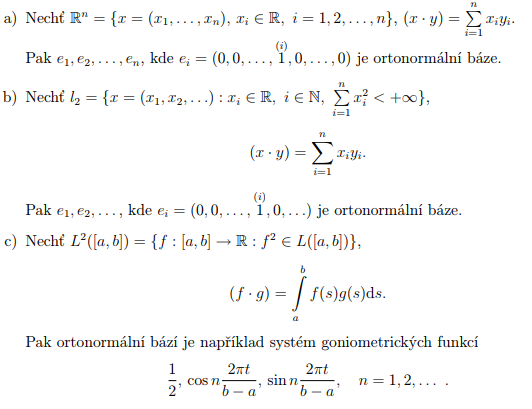
\includegraphics[width=0.8\textwidth]{Obrazky/priklady_prostoru}
\end{figure}


\section{Numerické metody řešení algebraických rovnic}  
\textit{reseni jedne nelinearni rovnice,reseni soustav nelin.rovnic,reseni soustav lin.rovnic(priame a iter.metody)}

\subsection{Riešenie soustav lineárních rovnic}  
\textit{Příme metódy} jsou takové, ktoré dodají v konečném počtu kroku přesné řešení (za predpokladu, že výpočet probíha bez zaokrouhlovacích chyb, teda zcela přesne).
\newline\textit{Iterační metódy} poskytují přibližné řešení, co je dostatoční pokud zachováme dobrou aproximaci řešení přesného. Počet kroku iterační metódy závisí na požadované přesnosti.
 \newline \newline Soustavou lin. rovnic rozumíme
\begin{align*}
a_{11} x_1 + a_{12} x_2 + \ldots + a_{1n} x_n &= b_1 \\
\ldots \\ 
a_{n1} x_1 + a_{n2} x_2 + \ldots + a_{nn} x_n &= b_n
\end{align*}
Danou soustavu je možný prepsat do tvaru $$ \sum_{j=1}^{n} a_{ij}x_j=b_i, \qquad i=1,2,...,n$$
 nebo v maticovém tvaru $$\textbf{Ax}=\textbf{b}.$$
Matici \textbf{A} nazýváme \textit{maticí soustavy}, \textbf{b} je \textit{vektor pravé strany} a  \textbf{x} je  \textit{vektor neznámých}. Budeme predpokládat, že matice soustavy je regulární, takže ťešena soustava má jediné řešení (Frobeniova veta).
 \subsection{Příme metódy}
\textbf{Gaussova eliminační metóda}

Základní příma metóda pro řešení soustav lin. rovnic je Gaussova eliminační metóda (dále GEM). Pozostáva ze dvou části-přímy a zpetný chod.
\newline V \textit{přímem chodu} GEM se soustava lin. rovnic převede na ekvivalentní soustavu $$\textbf{Ux}=\textbf{c},$$ kde \textbf{U} je tzv. \textit{horní trojuhelníková matice}, což je matice, ktorá má pod hlavní diagonálou všechny prvky nulové, tj. $u_{ij}=0$ pro $i\succ j$.
\newline     
$$U=\left( 
\begin{array}{ccc c r}
    u_{11} & u_{12} & u_{13} & ... & u_{1n} \\
    0 & u_{22} & u_{23} & ...  & u_{2n} \\
    0 & 0 & u_{33} & ... & u_{3n} \\
   \vdots & \vdots & \vdots & \vdots & \vdots \\
    0 & 0 & 0 & ... & u_{nn} \\ 
    \end{array} 
\right)$$


V \textit{zpetném chodu} se pak řeší soustava $$\textbf{Ux}=\textbf{c}.$$ Protože \textbf{A} je regulární, \textbf{U} je také regulární,z čeho vyplýva, že diagonální prvky jsou ruzne od nuly. Díky tomu vypočteme z poslední rovnice $x_{n}$, z předposlední $x_{n-1}$, atd.
\textbf{Přímy chod GEM}
Přímy chod má \textit{n-1} kroku (matice \textbf{A} má řád n). Matice \textbf{A} se mění každým krokem a to stejné vektor \textbf{b} co v k-tém kroku značíme $\textbf{A}^{(k)}$. V \textit{k-tém} kroku se snažíme vynulovat poddiagonální koeficienty v \textit{k-tém} sloupci matice $\textbf{A}^{(k)}$. Dosáhneme to tak, že od i-té rovnice odečteme $\textit{m}_{ik}$ násobek k-té rovnice lineární soustavy ($i\succ k$, protože jenom poddiagonální prvky)
$$a_{ik}^{(k)}-m_{ik}a_{kk}^{(k)}=0 \implies m_{ik}=\frac{a_{ik}^{(k)}}{a_{kk}^{(k)}}.$$
$a_{kk}^{(k)}$ se nazýva hlavní prvek nebo pivot-pokud se rovná nule, algoritmus zhavaruje (využitelný pouze když A je ryze diagonálne dominantní nebo pozitivne definitní).
\newline Tento algoritmus nevyužíva výběr hl.prvku (je braný diag.prvek), je však možní použít úplný výběr hlavního prvku nebo částeční výběr (většinou se používá částečný, kt. má menší počet operací a zaokrouhlovací chyby jsou stále dostatočne malý).
\newline 
\textit{Částečný výběr hl.prvku} v k-tém kroku eliminace se jako hl.prvek vybíra prvek s největši abs.hodnotou v zatím nezelimenované částí k-tého sloupca matice $\textbf{A}^{(k-1)}$ (prohodí se k-tý a r-tý řádek, $r\succ k$). Při \textit{Úplném výběru hl.prvku} se prohozují řádky i sloupce matice.
\newline GEM s částečným/úplným výběrem hl.prvku jsou dobře podmínené algoritmy za predpokladu, že matice soustavy je dobře podmíněná (protože velikost multiplikátoru nepřesahuje jedničku, vznikajíci zaokrouhlovací chyby se dalším výpočtem "nezesilují"). (asi by bolo vhodné niečo dodať o normách matíc a číslu podmíneností matic)
\textbf{LU rozklad}
Po ukončení přimého chodu dostaneme soustavu $\textbf{Ux}=\textbf{c}.$ Multiplikátory umístnime do dolní trojuhelníkové matice L.
$$
\bigg{[} l_{ik}= 
\begin{cases}
       0, & \text{pro } i=1,2,...,k-1 \\
       1, & \text{pro } i=k \\
        m_{ik}, & \text{pro } i=k+1,k+2,...,n
\end{cases}
\bigg{]}
$$

Platí: \textbf{A}=\textbf{LU}
\newline \textbf{Nasledujíci kroky:}
\newline 1) vypočteme soustavu $\textbf{Ly}=\textbf{b}$ pro neznámou y 
\newline 2) vypočteme soustavu $\textbf{Ux}=\textbf{y}$ pro neznámou x
\newline 3) soustava $\textbf{Ax}=\textbf{b}$ je ekvivalentní soustavě $\textbf{LUx}=\textbf{b}.$, takže x z 2) je naše řešení
\newline LU rozklad s částečným výběrem hl.prvku je založen na nájdení takových matic U (horní troj.matice),L (dolní troj.matice), P(permutační matice),že platí $\textbf{LU}=\textbf{PA}.$

\textbf{Choleského rozklad}
Platí: $\textbf{A}=\textbf{L}\textbf{L}^{T}$, kde \textbf{L} je dolní troj. matice jejíž prvky jsou ale definovane jinak než v u LU rozkladu. Postup pokračuje 1)-3) pro $\textbf{U}=\textbf{L}^{T}.$
\newline
\subsection{Iterační metódy}
Soustavu $\textbf{Ax}=\textbf{b}$ řešíme zvolením počátečního vektoru $\textbf{x}_{0}$ a generovaním posloupností vektoru $\textbf{x}_{1},\textbf{x}_{2}$,atd které konvergují k hlednanému řešení $\textbf{x}$. 
\newline\textbf{Konvergence}
\newline
řekneme, že iterační metóda konverguje, a píšeme $\textbf{x}_{k} \rightarrow\textbf{x}$, když  $\left\Vert\textbf{x}_{k}-\textbf{x}\right\Vert\rightarrow 0$. Chybu v k-té iteraci značíme $\textbf{e}_{k}=\textbf{x}_{k}-\textbf{x}$. Konvergence iterační metody z libovolného startovacího vektoru nastane, když konvergenční matice $\textbf{T}$ splňuje $\left\Vert\textbf{T}\right\Vert<1$, tahle podmínka se však neověřuje lehce.\newline Iterační metóda se ukončí když $\textbf{x}_{k}$ je dostačujíci aproximace \textbf{x}. Jedním z nejčastejších kritériií pro ukončení iterační metódy je  $\left\Vert\textbf{x}_{k+1}-\textbf{x}_{k}\right\Vert\leq \epsilon\left\Vert\textbf{x}_{k}\right\Vert$ pro dostatečne malé $\epsilon$.

\textbf{Jacobiova metoda}
\newline Matici \textbf{A} rozložíme ako \textbf{A}=\textbf{L+U+D}, kde\textbf{D} je diagonální matice, ktorá má stejnou diagonálu jako \textbf{A}, a kde \textbf{L}/\textbf{U} je ryze dolní/horní trojuholníková část matice \textbf{A}. Posloupnost vektoru $\textbf{x}_{k}$ je dána vztahem $$\textbf{D}\textbf{x}_{k+1}=\textbf{b}-\textbf{(L+U)}\textbf{x}_{k}.$$ Jacobiova metóda konverguje, když \textbf{A} je ryze diagonálně dominantní.

\textbf{Gauss-Seidelova metoda}\newline
Protože v Jacobiovej metode počítáme prvky vektoru  $\textbf{x}_{k+1}$ postupně jeden za druhým, vznikl nápad ihned využít ty složky  $\textbf{x}_{k+1}$, které jsou uz k dispozicií. Tak dostávamé Gauss-Seidlovu metodu. $$\textbf{(D+L)}\textbf{x}_{k+1}=\textbf{b}-\textbf{U}\textbf{x}_{k}.$$ MEtóda konverguje, když \textbf{A} je ryze diagonálně dominantní nebo pozitivne definitní. 
\newline Konvergence Gauss-Seidelovy metody je pro mnohé matice \textbf{A} rychlejší.

\textbf{Relaxační metody}\newline
Bezprostředně po vypočtení i-té složky v k+1 iteraci vektoru  $\textbf{x}_{k+1}$ provedeme její modifikaci $$\textbf{x}^{(k+1)}_i=(1-\omega)\textbf{x}^{(k)}_i+\omega\textbf{x}^{(k+1)}_i.$$
Relaxační parametr $\omega$ je volený tak, abychom vylepšili konvergenci základní metódy. Zvolíme-li $\omega=1$ dostávamé puvodní metodu, pro $\omega<1$ hovoříme o dolní relaxaci, v případě $\omega>1$ o horní relaxaci. Volba $\omega$ závisí na zvolené základní metodě a na matici soustavy $\textbf{A}$.

Inou známou iterační metodou je například metoda sdružených gradientu.
\subsection{Riešenie jednej nelineárnej rovnice}  
\subsection{Riešenie sústavy nelineárnych rovníc}  

\section{Interpolace a aproximace, numerické derivování a integrování}  

Aproximovat funkci $f(x)$ znamená nahradit ji funkcí $\varphi(x)$, která je k $f(x)$ v jistém smyslu blízká. Píšeme $\varphi(x)\approx f(x)$. Dva základní typy aproximace jsou interpolace a metoda nejmenších čtverců.

\textit{Interpolace} je aproximace, při níž $\varphi(x)$ nabývá v zadaných bodech $x_i$ předepsaných hodnot $y_i=f(x_i)$, někdy navíc žádáme, aby funkce $\varphi(x)$ a $f(x)$ měli v bodech $x_i$ také stejné derivace.

\textit{Metoda nejmenších čtverců} je aproximace, při níž $\varphi(x)$ "prokládáme" mezi zadanými body $[x_i,y_i]$ tak, aby "vzdálenost" funkcí $f$ a $\varphi$ byla v jistém smyslu minimální. Je přitom charakteristické, že funkce $\varphi$ neprochází body $[x_i,y_i]$.

\subsection{Interpolace}
Interpolační funkci $\varphi(x)$ vybíráme z vhodné třídy funkcí. Omezíme se na dva případy:
\begin{itemize}
\item  $\varphi(x)$ je polynom 
\item $\varphi(x)$ je po částech polynom, na každém subintervalu obecně jiný.
\end{itemize} 
\textbf{Interpolace polynomem}
Je zadáno $n$ navzájem různých bodů $x_0,x_1,...,x_n$, které nazýváme \textit{uzly interpolace} a v každém z nich je předepsaná hodnota $y_i$. Hledáme interpolační polynom $P_n(x)$ stupně nejvýše $n$, který splňuje interpolační podmínky $$P_n(x_i)=y_i,\quad i=0,1,...,n$$


\textbf{Lagrangeův tvar interpolačního polynomu}
$$P_n(x)=y_0l_0(x)+y_1l_1(x)+\ldots+y_nl_n(x)=\sum_{i=0}^{n}y_il_i(x),$$
kde $l_i(x)$ jsou tzv. fundamentální polynomy definované $$l_i(x)=\frac{(x-x_0)(x-x_1)...(x-x_{i-1})(x-x_{i+1})...(x-x_n)}{(x_i-x_0)(x_i-x_1)...(x_i-x_{i-1})(x_i-x_{i+1})...(x_i-x_n)}$$ z čeho vyplývá
\[
    l_i(x_k)= 
\begin{cases}
        1, & \text{pro } k=i\\
        0, & \text{pro } k\neq i
\end{cases}\quad  i,k=0,1,...,n,\\
\]
takže interpolační podmínky $P_n(x_k)=\sum_{i=0}^n y_il_i(x_k), \, k=0,1,\ldots,n$, jsou splněny. Interpolační polynom je daty $[x_i,y_i],\, i=0,1,\ldots, n$ určen jednoznačně, jelikož jsou-li $P$ a $Q$ interpolační polynomy splňující interpolační podmínky $P(x_i)=Q(x_i)=y_i$, pak polynom $P-Q$ je roven nule v uzlech $x_0,x_1,\ldots,x_n$ což je ve sporu s faktem, že polynom stupně $n$ může mít maximálně $n$ kořenů, pokud se nerovná identicky $0 \Rightarrow P-Q=0 \Rightarrow P=Q$. 
\newline Výhodou je jeho elegantní forma, hlavní nedostatky 
\begin{itemize}
\item Přidáme-li další uzel $x_{n+1}$, musíme přepočítat všechny fundamentální polynomy
\item Počet operací potřebných k výpočtu $P_n(\hat{x}) $ je poměrně značný, vyžaduje $2n^2+2n$ násobících operací a $2n^2+3n$ operací sčítacích.
\end{itemize}


\textbf{Newtonův interpolační polynom}\newline
Odstraňuje oba nedostatky Lagrangeového interpolačního polynomu.$$P_n(x)=a_0+a_1(x-x_0)+a_2(x-x_0)(x-x_1)+...+a_n(x-x_0)(x-x_1)...(x-x_{n-1})$$. Při přidání dalšího uzlu ostáva puvodní tvar interpolačního polynómu stejný a jenom se přičte nový člen. Koeficienty $a_i$ je možné vypočítat přímo z interpolačních podmínek nebo pomocí poměrné diference (lepší zpusob).

Poznámka k oběma interpolačným polynomum:Obecně nelze doporučit používaní interpolačních polynomu vysokých stupňu (jsou funkce, kde chyba interpolace raste s roustoucím počtem uzlu, Rungeova funkce), efektívnejší by bylo vhodne zormístnit uzly, avšak tuto možnost však obvykle nemáme, neboť uzly jsou pevně dané.

\textbf{Hermitova interpolace}\newline
Hlavní rozdíl pozostáva v tem, že interpolační polynom určují navíc také prědepsané derivace v uzlech. 
\newline
Nechť je každém uzlu zadáno $\alpha_i+1$ čísel $y_i^{(0)},y_i^{(1)},...,y_i^{(\alpha_i)}$. Označme $\alpha=n+\sum_{i=0}^n \alpha_i$. Pak Hermitovým interpolačním polynomem $P_alpha(x)$ nazveme polynom stupně nejvýše $\alpha$, který splňuje interpolační podmínky $$\frac{d^j}{dx^j}P_\alpha(x_i)=y_i^{(j)}\qquad j=0,1,...,\alpha_i,\quad i=0,1,...,n$$Je dokázáno, že existuje jediný takový polynom. Stejně jako u předchozích ani tady nelze obecně odporučit použití vysokého stupně polynomu.

\subsection{Interpolační splajny}
Když chceme interpolovat funkci $f(x)$ na poměrně dlhém intervalu $\langle a,b \rangle$, je vhodnejší nepoužívat interpolační polynomy vyšších stupňu ale interval rozdělit na řadu menších subintervalu a na každém z nich sestrojit interpolační polynom nižšího stupně. 
$$a=x_0 < x_1 < ... < x_{i-1} < x_{i} < {i+1} <...< x_{n-1} < x_n=b$$ je dělení intervalu $\langle a,b \rangle$. V každém uzlu $x_i$ je prředepsána hodnota $y_i$ interpolantu. Délka i-tého intervalu je $\langle x_{i-1},x_i \rangle$.
\subsection{Metoda nejmenších čtvercu}
\subsection{Numerické derivování}
\subsection{Numerické integrování}


\section{Numerické metody řešení počátečních problémú pro ODR}
Máme počáteční problém
\begin{align}
y'&=f(t,y(t)), \quad t \in [t_{0}, T], \\
y(t_{0})&=y_{0}
\end{align}
obecně je tento problém vektorový ($f:[t_{0},t_{f}]:\times\R ^{m} \rightarrow \R^{m}, \: y:\R \rightarrow \R ^{n}$, $y_{0}$ je vektor s m složkami) - jedná se tedy o soustavu.  Předpokládáme že problém je "well-defined", tj. řešení existuje a je jednoznačné (funkce $f$ je spojitá a  Lipschitzovská), a že existují derivace až do řádu, který budeme potřebovat. 

Rovnice vyšších řádů lze převést na soustavu rovnic prvního řádu. Proto nám stačí numerické metody pro řešení soustav rovnic prvního řádu.  

Analýza numerické metody je jednodušší pro skalární úlohu (rovnici), proto v následujícím bude vše děláno pro rovnici (stejně jako ve skriptech). 
\subsection{Základní pojmy}
\subsubsection*{Numerické řešení}
Numerické řešení jsou přibližné hodnoty hledaného řešení v bodech $t_{n}$, tj. posloupnost hodnost  $y_{0}, y_{1}, y_{2},...,y_{N}$. 

Interval $[t_{0}, T]$ na  kterém řešíme rovnici rozdělíme na N "dílků"
\begin{align}
t_{0} <  t_{1}< ... < t_{N} \leq T. 
\end{align} 
Hodnoty $t_{n}$ nazyvame \textbf{uzly}. 
Vzdálenost mezi dvěma uzly $t_{n}, t_{n+1}$ nazveme \textbf{délka kroku}: $h_{n}=t_{n+1}-t_{n}, \: n=0,1,...N-1$. Pokud jsou všechny délky kroku stejné $h_{n}=h,\; \forall n$ mluvíme o \textbf{rovnoměrném (ekvidistantním) dělení} a  platí vztahy
\begin{align}
h_{n}=h= \frac{T-t_{0}}{N}, \quad t_{n}=t_{0}+nh, \: n =0,1,...,N,
\end{align}
Pro získání řešení v jiných bodech než v uzlech musíme použít nějaký druh interpolace. 

\textbf{Značení:} \\
$y(t_{n})$ -- hodnota přesného řešení v bodě $t_{n}$ \\
$y_{n}$ -- hodnota aproximovaného (přibližného) řešení v bodě $t_{n}$

\subsubsection*{Numerická metoda}
Numerická metoda je předpis (algoritmus) pro postupný výpočet aproximací řešení   $y_{0}, y_{1}, y_{2},...,y_{N}$.

Krokem metody nazveme "přechod" od hodnoty $y_{n}$ k hodnotě $y_{n+1}$. \textbf{K-krokovou metodou} pak nazýváme metodu pro kterou výpočet $y_{n+1}$ závisí na \textit{k} předchozích aproximacích. Konkrétně pro jedno-krokovou metodu, $y_{n+1}$ závisí pouze na aproximaci $y_{n}$.

\subsection{Eulerovy metody a další pojmy numerické analýzy}
\subsubsection*{Explicitní Eulerova metoda}
  (dopředná eulerova metoda, anglicky: Euler method, explicit Euler method, forward Euler method)

Jedno z možných odvození je z Taylorova rozvoje
\begin{align}
y(t_{n+1}) = y(t_{n}+h)= y(t_{n})+hy'(t_{n}) + \frac{1}{2} h^{2} y''(\xi_{n}), \quad \xi_{n} \in (t_{n}, t_{n+1}).
\end{align}
Derivaci $y'$ nahradíme z rovnice $y'(t_{n})=f(t_{n},y(t_{n}))$ a když zanedbáme clen $\frac{1}{2} h^{2} y''(\xi_{n})$ dostaneme
\begin{align}
y(t_{n+1}) \approx y(t_{n})+h f(t_{n},y(t_{n})).
\end{align}
Přesné hodnoty $y(t_{n}), \, y(t_{n+1})$ nahradíme aproximovanými $y_{n}, y_{n+1}$ a dostaneme předpis Eulerovy metody
\begin{align}
y_{n+1}= y_{n} + hf(t_{n}, y_{n}).
\end{align}
Výpočet $y_{n+1}$ závisí pouze na jedné předchozí hodnotě aproximovaného řešení, tedy je to jednokroková metoda. Hodnota $y_{n+1}$ je určena explicitně, jedná se tedy o explicitní metodu. 

\subsubsection*{Chyby}
\textbf{Lokální diskretizační chyba} - $lte$ (local truncation error) je chyba, které se dopustíme v jednom kroku za předpokladu že $y_{n}$ je přesné řešení počáteční úlohy v čase $t_{n}$, tj. $y_{n}=y(t_{n})$:
\begin{align}
lte_{n}= y(t_{n+1})-y(t_{n})-h f(t_{n},y(t_{n})).
\end{align}
Z Taylorova rozvoje o kousek výš plyne, že $lte_{n}=\frac{h^{2}}{2} y''(\xi_{n})$ tedy $\vert lte_{n} \vert \leq C h^{2}$, kde $C=\frac{1}{2} \mathrm{max}_{t_{n}\leq t \leq t_{n+1}} \vert y''(t) \vert $. To je všechno moc pěkný - hlavní je, že lokální diskretizační chyba je úměrná velikosti kroku na druhou což označujeme pomocí Landauova symbolu jako $\mathcal{O}(h^{2})$.

Reálně tahle chyba nevzniká, protože předpoklad $y_{n}=y(t_{n})$ není obecně splněn (je splněn v prvním kroku a to jen pokud máme k dispozici přesnou počáteční podmínku). Tato chyba se tedy uplatňuje pouze při analýze vlastností metody.  

\textbf{Lokální chyba} - $le$ (local error)  je skutečná chyba které se dopustíme při reálném výpočtu v kroku od $t_{n}$ do $t_{n+1}$. S touto chybou pak pracujeme např. při řízení délky kroku.  $Le$ definovaná předpisem
\begin{align}
le_{n}=u_{n}(t_{n+1})-y_{n+1}
\end{align}
kde $u_{n}(t)$ je tzv. lokalni reseni pocatecniho problemu
\begin{align}
u'(t)=f(t,u_{n}(t)), \quad u_{n}(t_{n})=y_{n}.
\end{align}
Pokud zvolíme dostatečně malou délku kroku je rozdíl mezi $lte$ a $le$ prakticky zanedbatelný. 

\textbf{Globální diskretizační chyba} - $e$ (global truncation error) vzniká hromaděním lokálních chyb. 
\begin{align}
e_{n}= y(t_{n})-y_{n}.
\end{align}
Pro rovnoměrný dělení lze dokázat 
\begin{align}
\vert e_{n} \vert = \vert y(t_{n})-y_{n} \vert \leq C h,
\end{align}
což můžeme zase zapsat pomoci $\mathcal{O}(h)$ a řekneme, že Eulerova metoda je řádu (řádu přesnosti) 1. 

\textbf{Zaokrouhlovací chyby} asi nejsou žádným velkým překvápkem. Pokud tyto chyby nepřesáhnou $\varepsilon$ pak po $N$ krocích délky $h$ velikost nepřesáhne $K \varepsilon h^{-1}$, kde $K$ je konstanta nezávislá na $\eps$ a $ h$. Pak celková chyba $\approx Ch+ \eps K h^{-1}$. Reálně jsou zaokrouhlovací chyby malé takže pokud nepočítáme pro velmi velký počet kroků nemusí nás to nijak obtěžovat. 

\subsubsection*{Stabilita}
Počáteční problém
\subsubsection*{Implicitní Eulerova metoda}
Když opět vyjdeme z Taylorova rozvoje
\begin{align}
y(t_{n+1}-h)= y(t_{n}) = y(t_{n+1}) -hy'(t_{n+1})+ \frac{h^{2}}{2} y'' (\xi_{n}), \quad \xi_{n} \in (t_{n},t_{n+1}),
\end{align}
vypustíme člen $\frac{h^{2}}{2} y'' (\xi_{n})$ a použijeme rovnost $y'(t_{n+1})=f(t_{n+1},y(t_{n+1)}$, zaměníme přesné a aproximované hodnoty, dostaneme \textit{implicitní Eulerovu metodu}:
\begin{align}
y_{n+1}=y_{n}+h f(t_{n+1},y_{n+1}).
\end{align}
Hodnota $y_{n+1}$ je nyní dána implicitně rovnicí výše. Pro její určení musíme řešit obecně nelineární rovnici. 

Lokální diskretizační chyba je z Taylorova rozvoje výše  $\mathcal{O}(h^{2})$ a podobně jako u explicitní Eulerovy metody lze určit globální diskretizační chybu $\mathcal{O}(h)$. Obě Eulerovy metody jsou tedy řádu 1. 

Stabilita: 

vnějšek jednotkového kruhu se středem v bodě $[1,0]$. 

\subsubsection*{Lichoběžníková metoda}
Lichoběžníkovou metodu lze získat jako aritmetický průměr explicitní a implicitní Eulerovy metody:
\begin{align}
y_{n+1}= y_{n}+ \frac{1}{2} \left( f(t_{n},y_{n}) + f(t_{n+1},y_{n+1} \right).
\end{align}
$lte_{n} = \mathcal{O}(h^{3})$, $e_{n}= \mathcal{O}(h^{2})$ tj. metoda řádu 2. Oblast absolutní stability obsahuje celou zápornou polorovinu komplexní roviny. Interval absolutní stabilit je celá záporná reálná poloosa.  

\subsection{Explicitní Runge-Kuttovy metody}
Runge-Kuttovy (RK) metody jsou jednokrokové metody. S-stupňová explicitní RK metoda je určena předpisem
\begin{align}
k_{1}&= f(t_{n}, y_{n}) \\
k_{2}& = f(t_{n}+c_{2} h, y_{n} + a_{21} h k_{1}) \\
k_{3} &= f(t_{n}+c_{3} h, y_{n} + a_{31} hk_{1} + a_{32}h k_{2}) \\
\vdots& \\
k_{s} & = f(t_{n}+c_{s} h, y_{n} + a_{s1}h k_{1} + ... + a_{s, s-1}h k_{s-1})\\
y_{n+1}&= y_{n} + h(b_{1}k_{1}+b_{2}k_{2} + ...+ b_{s}k_{s}).
\end{align}
Koeficienty $k_{i}$ se nazývají  stupně. Koeficienty $a_{ij}, b_{i}, c_{i}$ určují konkrétní metodu. Lze je zapsat do tzv. Butcherovy tabulky:
\begin{center}  
 \begin{tabular}{r|r}
  $\textbf{c} $ & $\textbf{A} $ \\ \hline
  & $\textbf{b}^{T}$
   \end{tabular}
   \end{center}
   která pro explicitní metody vypadá následovně
   \begin{center}
 \begin{tabular}{l|lllll} 
   $0$      &     $0$        \\
  $ c_{2}$    &  $a_{2,1}$      &         \\
    $c_{3}$    &  $a_{3,1}$      &  $a_{3,2}$       & \\

    $\vdots$      & $\vdots $ & $\vdots$        \\
   $c_{s}$     &  $a_{s,1}$     &  $a_{s,2}$    & $\cdots$ &  $a_{s,s-1}$  &   \\\hline
    &$ b_{1}$        &$ b_{2}$  & $\cdots$   & $b_{s-1}$      & $b_{s} $\\      
  \end{tabular}  
\end{center}
První řádek, kde jsou jen nuly se někdy (třeba ve skriptech) vypouští. 

Stupně $k_{i}, i=1...,s,$ jsou směrnicí lokálního řešení procházejícího bodem $[t_{i}^{*},y_{i}^{*}]$, kde
\begin{align}
t_{i}^{*} = t_{n}+h c_{i}, \quad y_{i}^{*} = y_{n} +  a_{i1}h k_{1} + ... + a_{i, i-1}h k_{i-1}, \quad i=1,...,s.
\end{align}
Output $y_{n+1}$ je pak obdržen za pomoci lineární kombinace stupňů. Přesněji řečeno váženého průměru, protože součet všech $b_{i}$ je roven 1.

Pro odvození konkrétní metody si nejprve určíme počet stupňů metody. Poté vybereme koeficienty $a_{ij}, b_{i}, c_{i}$ tak aby metoda měla "dobrou" přesnost. Ta se měří pomocí lokální diskretizační chyby.\textit{ Metoda je řádu \textit{p} pokud pro lokální diskretizační chyba je řádu $\mathcal{O}(h^{p+1})$.} Pomocí toho lze odvodit podmínky řádu:
 \begin{align*}
 \sum _{j=1} ^{s}  b_{j} &= 1 \nonumber \\
 \sum _{j=1} ^{s}  b_{j}c_{j} &= \frac{1}{2}  \nonumber \\
 \sum _{j=1} ^{s} b_{j}c_{j}^{2}  &= \frac{1}{3} \nonumber \\
 \sum_{j=1} ^{s}  \sum _{k=1} ^{j-1} b_{j}a_{jk}c_{k}  &= \frac{1}{6} \nonumber
 \end{align*}
pro řád 1 - první rovnice, pro řád 2 - první a druhá, pro řád 3 - všechny čtyři. Pro vyšší řády počet podmínek roste (docela brutálně):
\begin{center}
\begin{tabular}{l|cccccccccc}
order $p$ & 1 & 2& 3& 4& 5&6&7&8&9&10 \\ \hline
number of conditions & 1 & 2& 4& 8& 17& 37& 85& 200& 486& 1205
\end{tabular}
\end{center}
(ta tabulka je tu spíš for fun, opovažte se to někdo učit).


Navíc se většinou předpokládá podmínka (většinou = vždycky, i když nutně ji splňovat asi nemusí všechny používaný metody ji splňují)
\begin{align}
c_{i}=\sum _{j=1} ^{i-1} a_{ij},\quad i=1,...,s.
\end{align}

Metody, které mají stejný počet stupňů jako je řád metody $s=p$ je možný sestrojit jen do řádu 4. Pro vyšší přesnost už potřebujeme $s > p$. Pro řádů 5 a 6 $s \geq p+1$ a pro vyšší pak $s \geq p+2$. 

\textbf{Metoda řádu 1} - explicitní Eulerova metoda, viz výše. 

\textbf{Metody řádu 2} - z podmínek řádu dostaneme, že koeficienty a,b jsou svázány podmínkou $b= \frac{1}{2a}$ pro $a\neq 0$. 
\begin{center}
\begin{tabular}{c|cc}
a & a \\ \hline
& 1-b & b
\end{tabular}
\end{center}
Těchto metod je kupa (dokonce nekonečně mnoho), takže takový ty proflákláknutý  který by bylo dobrý znát: \\
$a=\frac{1}{2}$ - modifikovaná Eulerova metoda, první modifikace Eulerovy metody (angl. midpoint Euler formula, explicit midpoint formula) \\
$a= 1$ - druha modifikace Eulerovy metody, Heunova metoda (angl. improved Euler method, Heun method) \\
$a=\frac{2}{3}$ - Ralstonova metoda 2. řádu. 

\textbf{Metody řádu 3} - např. Ralstonova metoda 3. řádu (základ metody Bogacki-Shampine o který bude řeč za dva/tři odstavce).

\textbf{Metody řádu 4} - nejznámější je klasická Runge-Kuttova metoda ("the" Runge-Kutta method, odvozená samotným W. Kuttou), super jednoduchá, má krásný koeficienty, proto byla dost populární před počítačové éře. Dneska už se používá spíš z nostalgie. 

\subsubsection*{Řízení délky kroku}

\subsubsection*{Odhad lokální chyby}
- Bogacki-Shampine 3(2), Dormand-Prince 5(4), Runge-Kutta-Fehlberg 4(5) \\
- metody s lokální extrapolací, FSAL property

\subsubsection*{Stabilita Runge--Kuttových metod}
Pokud řešíme testovací rovnici $y'=\lambda y,\; y(0)=1$ (viz u Eulerovy metody) RK metodou na rovnoměrném dělení s krokem $h$ dostaneme
\begin{align}
y_{n+1}=P_{s}(h \lambda) y_{n}
\end{align}
kde $P_{s}$ je polynom stupne s, určený pomocí konstant $b_{i}, a_{ij}$. Podmínka stability platí pouze pokud $h \lambda$ leží v oblasti absolutní stability $R_{A}$:
\begin{align}
h \lambda \in R_{A} = \lbrace z \in \mathbf{C} : \vert P_{s}(z) \vert < 1 \rbrace.
\end{align}
\textit{Explicitní RK metody mají omezenou oblast absolutní stability.} 

\subsection{Lineární mnohokrokové metody}
Tyto metody počítají přibližné řešení $y_{n+1}$ v uzlu $t_{n+1}$ z již spočtených aproximací $y_{n}, y_{n-1}, y_{n-2},...$ a odpovidajicich hodnot prave strany diferencialni rovnice. Tyto hodnoty jiz mame vypocteny, tedy pro ziskani $y_{n+1}$ s vysokou presnosti potrebujeme  jen malo novych vyhodnoceni prave strany. 

Predpis obecne linearni k-krokove metody:
\begin{align}
\alpha_{0} y_{n+1} + \alpha_{1} y_{n} + ... + \alpha_{k} y_{n+1-k} = h \left( \beta_{0} f(t_{n+1},y_{n+1})+ ... + \beta_{k}f(t_{n+1-k},y_{n+1-k}) \right)
\end{align}
Koeficienty $\alpha_{j}, \beta_{j}$ urcuji konkretni metodu. \\
Predpokladame normalizacni podminku $\alpha_{0}=1$ \\
Pokud $\alpha_{k} \neq0$ nebo $\beta_{k} \neq 0$ pak je metoda k-krokova \\
Pro $\beta_{0} \neq 0$ - implicitni metoda \\
Pro $\beta_{0}= 0 $ - explicitni metoda \\
Pro k-krokovou metodu potrebujeme $k-1$ startovacich hodnot $y_{0},y_{1},...y_{k-1}$, $y_{0}$ z pocatecni podminky, $y_{r}, r<k$ pomoci nejvyse r-krokove metody. 

\textbf{D-stabilita}
Řekneme, že metoda je stabilní ve smyslu Dahlquista (D-stabilní) jestliže všechny kořeny prvního charakteristického polynomu $\rho (\xi) = \xi^{k} + \alpha_{1} \xi^{k-1}+...+\alpha_{k-1} \xi+ \alpha_{k}$ leží uvnitř jednotkového kruhu $\vert z \vert < 1$ komplexni roviny $\mathbb{C}$ a pokud nektery koren lezi na hranici pak je jednoduchy. 

\textbf{Konvergence}
Uvažujeme D-stabilní lineárni mnohokrokovou metodu řádu $p \neq 1$ . Jestliže startovací hodnoty zadáme s chybou řádu $\mathcal{O}(h^{p})$ , pak globální diskretizační chyba je rovněž řádu $\mathcal{O}(h^{p}) $.

\textbf{Absolutni stabilita} = A-stabilita \\
Máme testovací úlohu (stejne jako pro RK metody)
\begin{align}
y'&=\lambda y \\
y_{0}&=1
\end{align}
na rovnomernem deleni pak pro linearni mnohokrokovou metodu dostaneme
\begin{align}
\sum_{j=0}^{k} (\alpha_{j} - h \lambda \beta_{j}) y_{n+1-j}=0
\end{align}
řešení pak hledáme ve tvaru $y_{n}=r^{n}$. Dosazenim do rovnice o kousek vys dostaneme
\begin{align}
\sum_{j=0}^{k}(\alpha_{j}-h \lambda \beta_{j})r^{n+1-j} = r^{n+1-k} \sum _{j=0}^{k} (\alpha_{j}-h \lambda \beta_{j}) r^{k-j}=r^{n+1-k} \pi (r,h\lambda) =0
\end{align}
kde 
\begin{align}
\pi(\xi,z) = \sum _{j=0}^{k}(\alpha_{j}-z \beta _{j}) \xi^{k-j}
\end{align}
je polynom stability. Oblast absolutni stability pro linearni mnoho krokove metody pak definujeme jako mnozinu bodu komplexni rovniny pro ktere kazdy koren $\xi$ polynomu stability $\pi(\xi, z)$ lezi uvnitr jednotkoveho kruhu komplexni roviny, $\vert \xi\vert<1$. A podminka stability plati pro $z$ z oblasti absolutni stability. 


\subsubsection*{Adamsovy metody}

Vezmu diferencialni rovnici
\begin{align}
y'(t)= f(t,y(t))
\end{align}
a zintegruju ji od $t_{n}$ do $t_{n+1}$
\begin{align*}
y(t_{n+1})-y(t_{n}) = \int \limits_{t_{n}}^{t_{n+1}} f(t,y(t) \mathrm{d}t
\end{align*}
Funkci $f(t,y(t))$ aproximujeme pomoci interpolacniho polynomu $P_{k-1}(t)$ stupne $k-1$ (Líba nepíše jakýho, lepší zdroje uvádí Langrangeův) tož tedy
\begin{align}
y(t_{n+1}) \approx y(t_{n}) + \int \limits _{t_{n}}^{t_{n+1}} P_{k-1}(t) \mathrm{d}t
\end{align}
kde hodnota iterpolacniho polynomu v uzlu interpolace je rovna funkcni hodnote prave strany diferencialni rovnice tj.:
\begin{align}
P_{k-1}(t_{n+1-j}) = f(t_{n+1-j},y(t_{n+1-j})).
\end{align}
Pak uz jen pribliznou rovnost nahradime rovnosti a presna reseni nahradime pribliznym resenim a voilà:
\begin{align}
y_{n+1}=y_{n}+ \int \limits _{t_{n}}^{t_{n+1}} P_{k-1}(t) \mathrm{d}t.
\end{align}

\textbf{Adams-Bashfothovy metody}
\\ dostanu ze vztahu vyse pro $j=1,2,..,k$. \\
Lze ji tedy zapsat jako \begin{align}
 y_{n+1}=y_{n} + h \sum _{j=1}^{k} \beta^{*}_{k,j} f(t_{n+1-j}, y_{n+1-j}),
\end{align}
kde koeficienty lze najit v tabulce ve skriptech nebo urcit z formule taktez ve skriptech (kdyby to nahodou nekoho zajimalo). 
 \\
D-stabilni \\
k-krokova  řádu k\\
AB1 je eulerova metoda \\

\textbf{Adams-Moultonovy metody}\\
dostanu ze vztahu vyse pro $j=0,1,2,..,k-1$. \\
Lze ji tedy zapsat jako \begin{align}
 y_{n+1}=y_{n} +h \beta_{k,0} f(t_{n+1},y_{n+1})+ h \sum _{j=1}^{k-1} \beta_{k,j} f(t_{n+1-j}, y_{n+1-j}),
\end{align}
zjevně jsou to metody implicitní \\
koeficienty viz skripta (pokud to nekoho zajima) \\
D-stabilní \\
pro $k=1$ jednokroková - prvniho radu \\
pro $k > 1$ (k-1)-krokova a radu k\\
AM1 - implicitni Euler, AM2 - trapezoidal

\textbf{Metody korektor-prediktor} \\
Schema PECE, P(EC)$^{s}$E, PECLE \\
ABk-AMk-PECE
\begin{itemize}
\item \textbf{P} = predikce - spocteme hodnotu $y^{*}_{n+1}$ ABk metodou 
\item \textbf{E} = evaluace - vyhodnotime pravou stranu $f^{*}_{n+1}=f(t_{n+1,y^{*}_{n+1}})$
\item \textbf{C} = korekce - spocteme hodnotu $y^{**}_{n+1}$ AMk metodou, hodnotu $y^{*}_{n+1}$ pouzijeme jako pocitacni aproximaci pro reseni nelinearni rovnice, tim nam staci jen nekolik malo iteraci
\item \textbf{E} = evaluace - vyhodnotime pravou stranu $f^{**}_{n+1}=f(t_{n+1,y^{**}_{n+1}})$
\end{itemize}

Muzeme take pouzit dvojci metod ABk-AM(k+1)

Algoritmus PECLE obsahuje navic krok zvany lokalni extrapolace. Pro dvojice ABk-AM(k) pouzijeme Milneův odhad  chyby 
\begin{align}
est_{n}=\frac{C_{k+1}}{C^{*}_{k+1}-C_{k+1}}(y^{**}_{n+1}-y^{*}_{n+1})
\end{align}
pro dvojice ABk-AM(k+1) pouzijeme
\begin{align}
est_{n}=y_{n+1}-y^{**}_{n+1},
\end{align}
kde $y_{n+1}$ je spocteno metodou AM(k+1)

ABk-AMk-PECLE
\begin{itemize}
\item \textbf{P} = predikce - spocteme hodnotu $y^{*}_{n+1}$ ABk metodou 
\item \textbf{E} = evaluace - vyhodnotime pravou stranu $f^{*}_{n+1}=f(t_{n+1},y^{*}_{n+1}mjj)$
\item \textbf{C} = korekce - spocteme hodnotu $y^{**}_{n+1}$ AMk metodou, 
\item \textbf{L} = lokalni extrapolace - spocteme $est_{n}$,  $y_{n+1}=y^{**}_{n+1}+est_{n}$
\item \textbf{E} = evaluace - vyhodnotime pravou stranu $f_{n+1}=f(t_{n+1},y_{n+1})$
\end{itemize}

\textbf{Metody zpetne diference}
- Metody zpetneho derivovani, BDF=backward differentiation formulas \\

V diferencialni rovnici
\begin{align}
y'(t_{n+1})=f(t_{n+1},y(t_{n+1}))
\end{align}
nahradime derivaci $y(t_{n+1})$ pomoci derivace $P'_{k}(t_{n+1})$ interpolacniho polynomu (Lagrange) stupne k, prochazejiciho body $[t_{n+1},y(t_{n+1})],[t_{n},y(t_{n})], [t_{n-1},y(t_{n-1})],...., [t_{n+1-k},y(t_{n+1-k})]$. 

Pak BDF metodu piseme ve tvaru
\begin{align}
\alpha_{k,0} y_{n+1} + \sum _{j=1}^{k}\alpha_{k,j} y_{n+1-j} = h \beta _{k,0}f(t_{n+1},y_{n+1})
\end{align}
implicitni \\
k-krokova  radu k \\
D-stabilini pro $k \leq 6$ \\
BDF1 = implicitni euler \\
Mají vetší chybové konstanty nez AM metody \\
Mají neomezenou oblast absolutní stability - BDF1 a BDF 2 jsou A-stabilní = jejich oblast absolutní stability obsahuje celou zápornou reálnou polorovinu, ostatní metody jsou $A(\alpha)$-stabilní = jejich oblast absolutní stability obsahuje nekonečný klín $W_{\alpha}=\lbrace re^{i \varphi} \in \mathbb{C} | r>0, \vert \varphi - \pi \vert < \alpha \rbrace$  - obrazky zde: $https://en.wikipedia.org/wiki/Backward\_differentiation\_formula$. \\
BDF metody jsou taky L-stabilni, L$(\alpha)$-stabilni 





\subsection{Tuhe problemy}

%%%%%%%%%%%%%%%%%%%%%%%%%%%%%%%%%%%%%%%%%%%%%%%%%%%%%%%%%%%%%%%%%%%%%%%%%%%%%%%%%%%%%%%%%%%%%%%%%%%%%


\section{Prostory funkcií}

\section{Numerické metody řešení okrajových problémú ODR}
metoda střelby, diferenční metoda, metoda konečných objemů, metoda konečných prvků

\section{Numerické metody řešení PDR}
diferenční metoda, metoda konečných objemů, metoda konečných prvků
